% !TeX spellcheck = es
\documentclass[11pt, titlepage]{article}

\usepackage[spanish,mexico]{babel}
\usepackage{xcolor}
\definecolor{darkblue}{rgb}{0.1 , 0.1, 0.7}
% referencias antes de geometría!
\usepackage[
hyperfootnotes=true,
urlcolor=blue,
colorlinks=true,
linkcolor=darkblue,
citecolor=darkblue]{hyperref}

% Texto matemático
%\usepackage[utf8]{inputenc}
\usepackage[a4paper,top=2cm,bottom=2cm,left=3cm,right=3cm,marginparwidth=1.75cm,headheight=28pt]{geometry}
%\usepackage[spanish, mexico]{babel}
\usepackage{graphicx}

%\usepackage[utopia]{mathdesign}
\usepackage[T1]{fontenc}					
\usepackage[utf8]{inputenc}		
%\renewcommand*\familydefault{\sfdefault} 


\usepackage{amsmath,array,IEEEtrantools,bm}
\usepackage{pdfpages}
% ENCABEZADO
\usepackage{fancyhdr,framed}
\setlength{\headheight}{44pt}
\pagestyle{fancy}
% TODO
\usepackage[
textwidth=2.6cm,
textsize=footnotesize,
]{todonotes}

\usepackage{natbib}
\usepackage{afterpage}
% !TeX root = ../main.tex



%% ROCKET
\newcommand{\CG}{{\mathrm{CG}}}
\newcommand{\LCG}{L_\CG}
\def\equilibrium{\mathrm{eq}}


%% DIFFERENTIAL OPERATOR
\makeatletter
\providecommand*{\diff}%
{\@ifnextchar^{\DIfF}{\DIfF^{}}}
\def\DIfF^#1{%
	\mathop{\mathrm{\mathstrut d}}%
	\nolimits^{#1}\gobblespace}
\def\gobblespace{%
	\futurelet\diffarg\opspace}
\def\opspace{%
	\let\DiffSpace\!%
	\ifx\diffarg(%
	\let\DiffSpace\relax
	\else
	\ifx\diffarg[%
	\let\DiffSpace\relax
	\else
	\ifx\diffarg\{%
	\let\DiffSpace\relax
	\fi\fi\fi\DiffSpace}

%% CONTROL:
\newcommand{\dimfont}[1]{\ensuremath{#1}}
\newcommand{\Cme}[1]{\mathbf{#1}}
\newcommand{\Mme}[1]{\mathbf{#1}}
\newcommand{\Nme}[1]{\mathrm{#1}}
\newcommand{\Ts}{T_s}

\newcommand{\eye}{\Mme{I}}
%transpose
\def\dt{\Delta t}
\def\tp{\!^{\top}\!}
% Small
\def\MA{\Mme{A}}
\def\MB{\Mme{B}}
\def\MC{\Mme{C}}
\def\MD{\Mme{D}}
\def\ME{\Mme{E}}

\def\MQ{\Mme{Q}}
\def\MR{\Mme{R}}
\def\MK{\Mme{K}}
\def\MW{\Mme{W}}
\def\MX{\Mme{X}}
\def\MV{\Mme{V}}
\def\ctrb{\Mme{Y}}
\def\Mzero{\Mme{0}}
\def\obsv{\Mme{\mathcal{O}}}

\newcommand{\ts}[2]{\left. #1\right|_{ #2}}

\def\error{\varepsilon}
\def\Cx{\Cme{x}}
\def\Cf{\Cme{f}}
\def\Cy{\Cme{y}}
\def\Cu{\Cme{u}}
\def\Cn{\Cme{n}}
\def\Cd{\Cme{d}}
\def\Czero{\Cme{0}}
\def\Cv{\Cme{v}}
\def\Cz{\Cme{z}}
\def\Cw{\Cme{w}}

\def\Jcost{\Cme{\mathcal{J}}}
% RK4
\def\Ca{\Cme{a}}
\def\Cb{\Cme{b}}
\def\Cc{\Cme{c}}


\def\noise{{n}}
\def\disturb{{d}}
\newcommand{\di}{\ensuremath{\textrm{d}}}

\newcommand{\Matlab}{{\sc Matlab}}

\def\matdiv{\bm{\textbackslash}}

\newcommand{\spartial}[2]{\frac{\partial {#1}}{\partial {#2}}}
\newcommand{\dpartial}[2]{\frac{\partial^2 #1}{\partial #2 ^2}}

%# ROBUST
\def\lap{\mathcal{L}}
\newcommand\lapc[1]{\lap \left\{#1\right\}}
\newcommand\ilapc[1]{\lap^{-1} \left\{#1\right\}}
\def\xbar{\bar{x}}
\def\ubar{\bar{u}} 

\def\MP{\Mme{P}}
\def\ML{\Mme{L}}
\def\MT{\Mme{T}}
\def\MS{\Mme{S}}


\def\Cr{\Cme{r}}
\def\Cn{\Cme{n}}

\def\openloop{{\textrm{\tiny{LA}}}}
\def\closedloop{{ \textrm{\tiny{LC}}}}
\def\true{{ \textrm{\tiny{real}}}}

% RIGID BODY MECHANICS
\newcommand{\frm}[1]{\mathrm{#1}}  % Frame of reference
\newcommand{\ogn}[1]{\mathcal{#1}} % Frame origin / point of reference
\newcommand{\skw}[1]{\tilde{#1}}   % skew matrix notation
\newcommand{\uveci}{{\bm{\hat{\textnormal{\bfseries\i}}}}}
\newcommand{\uvecj}{{\bm{\hat{\textnormal{\bfseries\j}}}}}
\DeclareRobustCommand{\uvec}[1]{{% Unit length vector of arbitrary orientation
		\ifcsname uvec#1\endcsname
		\csname uvec#1\endcsname
		\else
		\bm{\hat{\mathbf{#1}}}%
		\fi
}}
\DeclareRobustCommand{\avec}[1]{{%
		\underline{#1} %		\bm{\mathbf{#1}}%
}}
\DeclareRobustCommand{\bvec}[1]{{% Orthogonal basis vector
%		\ifcsname bvec#1\endcsname
%		\csname bvec#1\endcsname
%		\else
		\bm{\hat{\mathbf{#1}}}%
%		\fi
}}
\def\tform{\mathbf{A}}
\newcommand{\transform}[1]{\tform^\frm{#1}}
\newcommand{\dottransform}[1]{\dot{\tform}^\frm{#1}}
\def\attitude{\mathbf{H}}
\newcommand{\inertia}[2]{J_{\ogn{#1}}^{\frm{#2}}}
\newcommand{\inertiarotor}[2]{\inertia{\!\mathrm{r}#1}{#2}}


\makeatletter
\newcommand*\bigcdot{\mathpalette\bigcdot@{.5}}
\newcommand*\bigcdot@[2]{\mathbin{\vcenter{\hbox{\scalebox{#2}{$\m@th#1\bullet$}}}}}
\makeatother

% THEOREMS/ EXERCISES
\usepackage{amsthm}
\theoremstyle{definition}
%\newtheorem{definition}{Definition}[chapter]
%\newtheorem{theorem}{Teorema}[chapter]
%\newtheorem{exercise}{Ejercicio}[chapter]
%\usepackage{bigfoot} % to allow verbatim in footnote
\usepackage[numbered,framed]{matlab-prettifier}



\let\ph\mlplaceholder % shorter macro
\lstMakeShortInline"
\renewcommand{\lstlistingname}{Código}
\renewcommand{\lstlistlistingname }{Códigos \Matlab}
\lstset{
  style              = Matlab-editor,
  basicstyle         = \mlttfamily,
  escapechar         = ",
  mlshowsectionrules = true,
  numbers = none,
  tabsize=4,
  literate = {-}{-}1,
}
\lstnewenvironment{sflisting}[1][]
{\lstset{#1}\mathversion{sans}}{}

% !TeX root = ../pf-cretton-whitti.tex
\usepackage{amssymb}
\usepackage{alphalph}

\makeatletter
\newcommand*{\myfnsymbolsingle}[1]{%
	\ensuremath{%
 		\ifcase#1% 0
 		\or % 1
 		*%   
 		\or % 2
 		\dagger
 		\or % 3  
 		\ddagger
 		\or % 4   
 		\mathsection
 		\or % 5
 		\mathparagraph
 		\or
 		\lozenge
 		\or
 		\aleph
 		\or
 		\backepsilon
 		\or
 		\flat
 		\or 
 		\maltese
 		\or
 		\circledast
 		\or
 		\gimel
 		\or
 		\wp
 		\else % >= 7
 		\@ctrerr  
 		\fi
	}%   
}   
\makeatother

\newcommand*{\myfnsymbol}[1]{%
	\myfnsymbolsingle{\value{#1}}%
}

% remove upper boundary by multiplying the symbols if needed
\newalphalph{\myfnsymbolmult}[mult]{\myfnsymbolsingle}{}

\renewcommand*{\thefootnote}{%
	\myfnsymbolmult{\value{footnote}}%
}


\renewcommand*{\thefootnote}{%
	\myfnsymbolmult{\value{footnote}}%
}

\usepackage[sort=none,abbreviations]{glossaries-extra}
\setabbreviationstyle{long-short}

\newglossaryentry{corrutina}
{
	name=Corrutina,
    text=corrutina,
	description={Una unidad de procesamiento que puede ejecutarse en simultaneo con otras corrutinas.}
}

\newglossaryentry{lqr}
{
	name=Linear Quadratic Regulator,
	text=LQR,
	description={Regulador basado en control óptimo que busca reducir error cuadratico de una función costo.}
}

\newabbreviation{i2c}
{I$^2$C}
{Protocolo de comunicación de dos hilos que permite comunicar varios circuitos integrados en un bus.}

\newabbreviation{gpio}
{GPIO}
{Salida digital de uso genérico. Pueden estar en \emph{high} (tensión de fuente) o \emph{low} (puesto a tierra).}

\newabbreviation{spi}
{SPI}
{Serial peripheral interface. Un protocolo de comunicación full-duplex de Motorola.}

\newabbreviation{uart}
{UART}
{Protocolo de comunicación universal asincrono.}

\lhead{ LIA}
\newcommand{\mldivide}{\,{\boldsymbol{\backslash}}\,}
\usepackage{pdfpages}
\author{Patricio Whittingslow \and Luis Cretton}
\begin{document}
\begin{titlepage}
	
	\centering
	{\small LIA Aerospace \par}
	
	
	\vspace{8cm}
	{\Huge Gimballed EDF propelled VTVL vehicle design and control  \par}
	\vspace{2cm}
	{ \large {
			Patricio Whittingslow \\ Luis Cretton 
		\par}}
	\vspace{4cm}
	\today
	
\end{titlepage}

\begin{abstract}
	Un resumen debería no incluir referencias y no superar 250 palabras.
\end{abstract}

\newpage
\tableofcontents
\newpage
\printunsrtglossaries
\vfill
\hrule
\vspace{-1cm}
\subsection*{Nota del autor}
Si el documento es abierto desde un lector PDF moderno (Chrome, Adobe Acrobat Reader, entre otros), se podrá navegar el mismo mediante las referencias (haciendo click derecho).
\newpage

\section{Introducción}
El diseño, desarrollo, fabricación, armado, simulación y lanzamiento de cohetes, no es una tarea
sencilla ni repetida en intervalos de cortos de tiempo, al contrario, suelen llevar décadas y una
fuerte inversión para que sean posibles estos logros. El diseño y auge de vehículos VTVL viene
a subsanar estos factores ya que una vez terminada la misión el vehículo se puede reutilizar,
con mínimas intervenciones, y estaría listo para una nueva misión, atacando estos dos puntos principales anteriormente mencionados, el tiempo y el costo. Esto difiere del método convencional donde el vehículo, luego de completar la misión, pasa a formar parte de basura espacial o, en el mejor de los casos, es recuperado del mar como el caso del Space Shuttle. 

\medskip

Un vehículo VTVL es aquel que despega verticalmente (como la mayoría de los cohetes
convencionales) y aterriza verticalmente, por sí solo sin necesidad de ser tripulado, y con el
objeto de completar una misión, esto supone una gran variante de ventajas, como ser una de
las más destacadas el reutilizamiento del vehículo, con todo lo que ello implica, logrando una
optimización de los costos, disminución de huella ecológica, y tiempo de desarrollo para las empresas interesadas. %%

\medskip

Los vehículos VTVL son tan viejos como el primer alunizaje. Traen en si varias ventajas frente a otros vehículos voladores como la gran reducción de espacio necesario para despegar y aterrizar. Esto no es un detalle menor dado que la mayor parte de la superficie terrestre de la tierra no son pistas de aterrizaje si no más bien terreno formado naturalmente.

\medskip

Este documento propone el diseño, simulación, control y fabricación de un vehículo con capacidades VTVL siendo un prototipo de baja escala. 
Este prototipo serviría como punta pie inicial
para vehículos de escala mayor que puedan completar misiones espaciales. Existen varias ventajas de implementar este tipo de tecnología.

\medskip

A baja escala, un vehículo que despega y aterriza por su cuenta, teniendo la capacidad de
superar obstáculos que se presenten, puede ser de gran utilidad en ambientes hostiles para el
ser humano, que esto se logre de manera rápida y efectiva podría ser la diferencia entre el
éxito o no de la misión.
Como ser el transporte de insumos médicos en tiempo real desde que un paciente lo requiere,
en zonas de acceso limitado.

\medskip

En la última década hay un interés renovado en imágenes espaciales. El vehículo podría adquirir imágenes para fines de sistemas de monitoreo y análisis geoespacial como hacen las empresas \textit{Ceres Imaging} y \textit{Satellogic}. %de una situación en la que no se disponga del tiempo suficiente para el accionar convencional a bajas velocidades como ser un helicóptero o un dron.  

\medskip

El vehículo una vez desarrollado y funcionando, puede servir de plataforma para diversos
estudios de fenómenos de dinámica de fluidos, como ser, mediciones aerodinámicas,
investigación del \textit{fuel sloshing} en vehículos con tanques esbeltos.

\medskip

El vehículo provee la capacidad de testear sistemas de control a escala pequeña que en caso de devenir en una falla, el costo total de perdidas seria mucho menor con respecto a un vehículo mas grande con sistemas caros y complejos.  Al tener un sistema de control definido en términos de parámetros del vehículo, se puede escalar para luego ser probado en un vehículo mas grande. Al ser también un sistema más chico y manipulable qué el vehículo de escala grande, tornándose más fácil las pruebas y los problemas de software y hardware de vuelo.

\medskip


Los sistemas de vehículos orbitales tienen sistemas complejos que deben ser testeados en una primera etapa mediante algún ensayo controlado. El vehículo que se desarrolla en el presente documento podría ser usado para tales fines como una plataforma para pruebas como ser el despliegue de una nariz o etapa, comprobación de sensores y actuadores a gran velocidad y con empuje variable.


\section{Estudios}
En lo que se refiere a la construcción del vehículo, el diseño propuesto paso por varias etapas y
decisiones de ingeniería hasta su forma final. Desde su diseño en lápiz y papel hasta la
simulación del CAD con el detalle del ultimo bulón del ensamble para ser cargado al sistema de control en la forma de una matriz de inercia, centro de masa y dinámicas de vuelo, e ir en paralelo retroalimentándose con estos parámetros. En base a esto se realizaron modificaciones sobre el código de control y las simulaciones.


\subsection{Agua como propelente}\label{ssec:propAgua}
El primer prototipo muy distante del diseño final perteneciente a este trabajo, consistía en un
recipiente a presión con agua, abulonado a un chasis, con un cardán y actuadores para poder redirigir el
empuje. 

\medskip

La figura~\ref{fig:bottlerocket} muestra los resultados de una simulación de un vehículo pequeño de aluminio con un recipiente a presión lleno en parte de agua y aire a 200 bar. La simulación considera masa variable y una transición isoentrópica del gas en el recipiente. En el mejor de los casos se llegaba a un tiempo de vuelo cercano a los 4 segundos, que no era adecuado para comprobar el sistema de control en nuestras condiciones. 

Para optimizar este problema se modificaba

\begin{itemize}
    \item Diámetro de la tobera -- más empuje vs. menos tiempo de vuelo controlado
    \item Volumen de agua -- más tiempo de vuelo vs. mayor peso de vehículo
\end{itemize}


\begin{figure}[!ht]
    \centering
    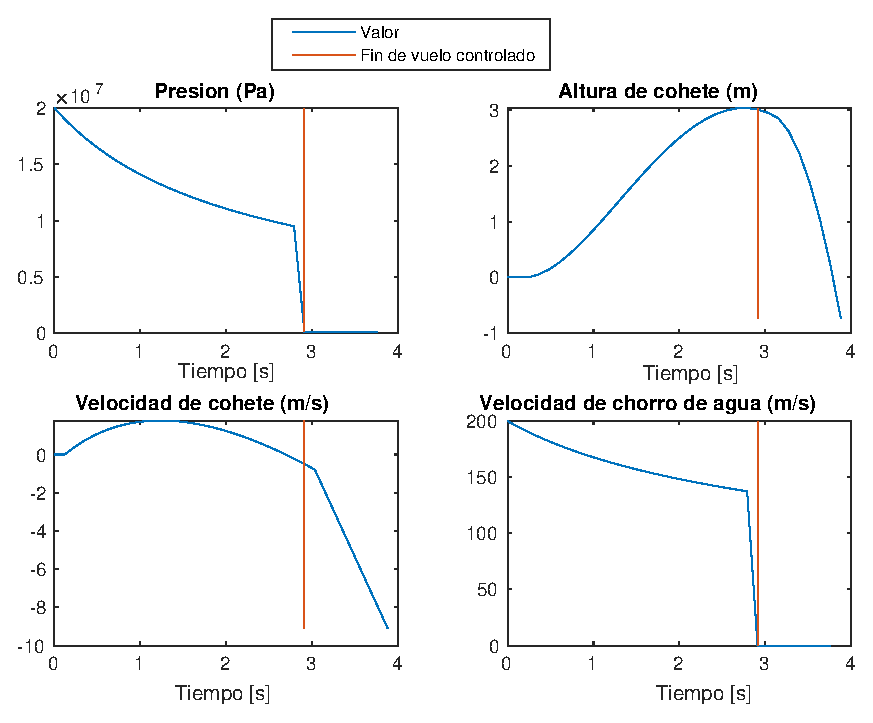
\includegraphics[width=0.8\linewidth]{fig/bottlerocket}
    \caption{Análisis preliminar para un vehículo propulsado por agua a presión. La presión es la del tanque (absoluta). El peso estructural que se utilizó fue de 10kg.}
    \label{fig:bottlerocket}
\end{figure}

Esto representa un vuelo de gran aceleración inicial, de mucha violencia, que dificulta la comprobación de sistemas en el que se tienen que tunear varios los parámetros de control y resolver los problemas de hardware que se vaya presentando. 

\subsection{Turbina a reacción}\label{ssec:turbina}
Se propuso la construcción de una turbina de combustible líquido, como método de propulsión
del vehículo favorable debido al excelente cociente de peso-empuje.

Esta idea se vio descartada por la pandemia que estamos atravesando (COVID19) debido a que
no teníamos acceso al taller de la institución para poder realizar en tiempo y forma el
dispositivo mecánico, que era la primer tarea inmediata a tener en banco de pruebas
asegurando su funcionamiento en optimas condiciones, para luego proseguir con el desarrollo
del vehículo y el sistema de control.


\subsection{Propulsión eléctrica}\label{ssec:propelectrica}


\begin{figure}[htb]
    \centering
    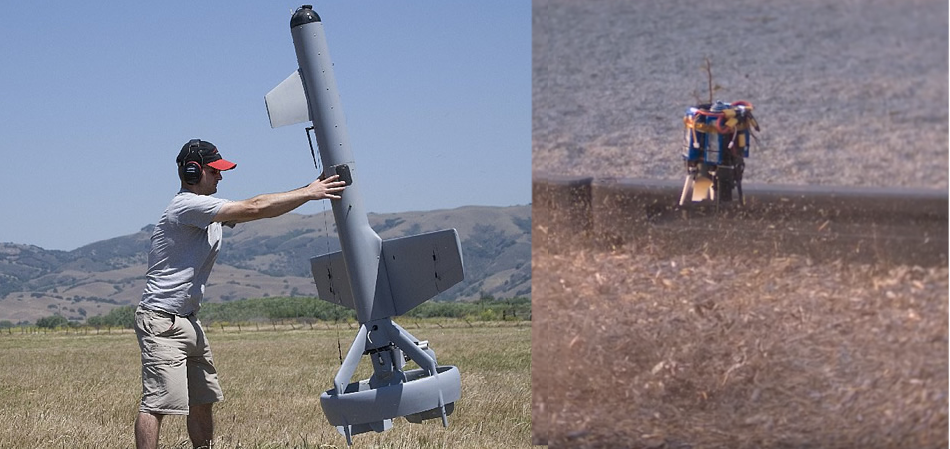
\includegraphics[width=0.8\linewidth]{fig/vbat_icarus.png}
    \caption{Dos vehículos VTVL eléctricos modernos. ``VBat'' (Izq.) y ``\href{https://hackaday.com/2018/08/31/single-rotor-drone-a-thrust-vectoring-monocopter/}{Ikarus}'' (Der.).}
    \label{fig:vbat_icarus}
\end{figure}

Luego de descartar las ideas vistas en~\ref{ssec:propAgua} y~\ref{ssec:turbina} se pasó al análisis de la incorporación de una turbina eléctrica que es un dispositivo ya existente en el mercado, no en nuestro país, pero que podría llegar a importarse teniendo en cuenta la pesificación del valor de los componentes en el exterior y los diversos costos asociados a la entrada al país de los mismos, se contemplo desde ese entonces la financiación privada, que la proveyó LIA Aerospace.\footnote{Agradecemos a \gls{lia} por hacerse cargo de la compra de los componentes faltantes que cayeron fuera del presupuesto necesarios para la fabricación del cohete.} 

Dadas las limitaciones de tiempo y alcance de un proyecto de la universidad se decidió por un diseño compuesto por elementos comercialmente disponibles.\footnote{\textit{Commercial off the shelf} (COTS)}

\medskip

Para lograr estas tareas los vehículos VTVL de baja escala generalmente son propulsados por motores eléctricos, como es el caso del proyecto FROG de la ESA.\todo{AGREGAR CITA}

\medskip

Los vehículos VTVL eléctricos son propulsados por hélices en su mayoría y constan casi siempre de 3 o más propulsores en un arreglo simétrico y plano. Recientemente hay un interés por la construcción de vehículos de una sola hélice por la buena relación empuje--peso que tienen. Sin embargo, estos vehículos no vienen sin sus complicaciones: 

\begin{itemize}
    \item La rotación dada al aire por la hélice causa un momento en el eje de propulsión que puede ser contrarrestado en vehículos multirrotores.
    \item Inclinar al rotor durante su funcionamiento causa una fuerza perpendicular a la dirección de inclinación conocido como el efecto giroscópico. 
\end{itemize}

El primer punto puede ser mitigado agregando álabes a la salida del chorro para enderezar el flujo y contrarrestar la rotación. El segundo punto se resuelve conociendo las ecuaciones de momento angular y controlando actuadores con un sistema de control a lazo cerrado. Los sistemas vistos en la figura~\ref{fig:vbat_icarus} suelen tener la particularidad de poder ser representados con relativa facilidad usando un solo marco de referencia sobre el vehículo para calcular las ecuaciones de momento angular.

\medskip

Existen placas pre-programadas para vehículos multirrotores, pero en el caso de vehículos monorrotores de hélice fija se precisa re-programar la placa para compensar por el efecto giroscópico y agregar dinámica de álabes ya que no hay software disponible aún para esta configuración. En el caso de tener una hélice móvil se suma un nivel de complejidad agregada debido al despeje de las ecuaciones de momento angular (ver sección~\ref{sec:ecuacionesRigid}). Al momento de escribir este documento aún no hay desarrollo disponible de carácter público para esta configuración.


\section{Modelo 2D simplificado} \label{sec:model2d}

Esta siguiente sección detallará el tratamiento matemático efectuado para controlar un vehículo con propulsión vectorizada en el plano. El propósito es ilustrar a un nivel simple las herramientas que se aplicaron para controlar el vehículo diseñado.

\begin{figure}[htb!]
	\centering
	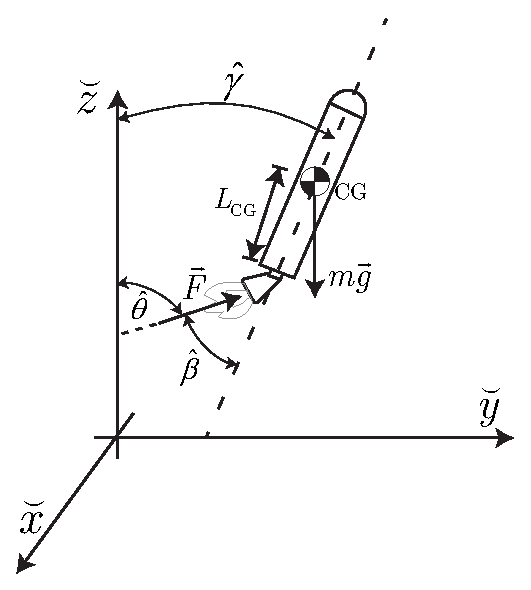
\includegraphics[width=9cm]{fig/rocketFBD.eps}
	\caption{Diagrama de cuerpo libre de un vehículo con propulsión vectorizada 2D.}
	\label{fig:FBD2D}
\end{figure}


\subsection{Modelado matemático}
Se comenzó con las ecuaciones dinámicas de un vehículo en el plano con control de propulsión vectorizada (por ángulo)

\[
\left\{
\begin{array}{l}
	\ddot{y}=\frac{F}{m} \sin(\gamma+\beta) \\
	\ddot{z}=\frac{F}{m} \cos (\gamma+\beta)-g \\
	\ddot{\gamma} = \frac{L_{\CG}\cdot F}{I_{xx}}\sin\beta
\end{array}
\right.
\]
donde \(\LCG\) y \(F\) están en función del tiempo, $m =m_0 - \int \dot{m} $ y $\theta = \gamma+\beta$. 

Vale la pena aclarar que no se tomaron en cuenta los siguientes efectos:
\begin{itemize}
	\item Viento y efectos aerodinámicos
	\item \textit{Fuel sloshing}
	\item Efectos relativistas
\end{itemize}

\subsection{Armado de sistema lineal}

Se propuso un punto de operación alrededor del cual se efectuó la linealización de las ecuaciones. El estado del vehículo alrededor del cual se linealizó fue \textit{vertical y quieto en el espacio}.\footnote{La linealización es valida solo para un vehículo vertical. Se deberá modificar el método para modelar un vehículo orbital.} 

\begin{align*}
	\gamma^* = 0 \\
	\beta^* = 0 \\
	F^* = mg
\end{align*}
en este caso $F$ fue la desviación del punto de operación siendo $\Delta F = F- mg$.

\subsection{Representación en espacio de estados}
El número de variables de estado fue igual a número de almacenadores de energía independientes. Estos son

\begin{enumerate}
	\item[$z$] Energía potencial por la gravedad
	\item[$\dot{y},\dot{z}$] Energía cinética del vehículo
	\item[$\dot{\gamma}$] Momento angular del vehículo
\end{enumerate}
entonces, las variables de estado fueron las siguientes
\begin{align*}
	x_1 = y \\
	x_2 = \dot{y} \\
	x_3 = z \\
	x_4 = \dot{z} \\
	x_5 = \gamma \\
	x_6 = \dot{\gamma}
\end{align*}
donde $\dot{x_1} = x_2$, $\dot{x_3} = x_4$ y $\dot{x_5} = x_6$

Se aprovecho la expansión de Taylor para la linealización de expresiones trigonométricas:
\[
\sin(x+y)|_{x=x_0+\Delta x,y=y_0+\Delta y} \approx \sin(x_0+y_0) + \cos(x_0 + y_0) (x-x_0) + \cos(x_0 + y_0) (y-y_0)
\]
\todo{Revertir cambios tiempo pasado}
Las ecuaciones dinámicas de los estados 2,3, y 4 fueron dadas por las ecuaciones mostradas al comienzo de esta sección.

Abajo se encuentran las ecuaciones de estados
\begin{equation}
	\dot{x_2} = \frac{F}{m} \left( \gamma+\beta \right) = g x_5 + g u_2 
\end{equation}
\begin{equation}
\dot{x_4} = \frac{F}{m} - g =\frac{F-F_0}{m}= \frac{u_1}{m}
\end{equation}
\begin{equation}
\dot{x_6} = \frac{\LCG \cdot F}{I_{xx}} \beta = \frac{\LCG \cdot mg}{I_{xx}} u_2 
\end{equation}

donde $\Ts$ es el periodo de muestreo.

Los vectores de entrada y salida resultaron
\[
\Cme{u}(t) = \begin{bmatrix}
u_1 \\
u_2
\end{bmatrix} = \begin{bmatrix}
\Delta F \\
\beta
\end{bmatrix}
\]
\[
\Cme{y}(t) = \begin{bmatrix}
y_1 \\
y_2 \\
y_3
\end{bmatrix} = \begin{bmatrix}
y \\
z \\
\gamma
\end{bmatrix}
\]
tal que las ecuaciones de salida son

\begin{equation}
	y_1 = x_1 
\end{equation}
\begin{equation}
	y_2 = x_3
\end{equation}
\begin{equation}
	y_3 = x_5
\end{equation}

Se calcularon las matrices del sistema y de control ($\Mme{D} = [0]$)
\begin{equation} \label{eq:ssmatrices}
	\Mme{A} = 
	\left[\begin{array}{cccccc} 0 & 1 & 0 & 0 & 0 & 0\\ 0 & 0 & 0 & 0 & g & 0\\ 0 & 0 & 0 & 1 & 0 & 0\\ 0 & 0 & 0 & 0 & 0 & 0\\ 0 & 0 & 0 & 0 & 0 & 1\\ 0 & 0 & 0 & 0 & 0 & 0 \end{array}\right],\quad \Mme{B} = 
	\left[\begin{array}{cc} 0 & 0\\ 0 & g\\ 0 & 0\\ \frac{1}{m} & 0\\ 0 & 0\\ 0 & \frac{\LCG \cdot mg}{I_{xx}} \end{array}\right], \quad \Mme{C} =  \left[\begin{array}{cccccc} 1 & 0 & 0 & 0 & 0 & 0\\ 0 & 0 & 1 & 0 & 0 & 0\\ 0 & 0 & 0 & 0 & 1 & 0 \end{array}\right]
\end{equation}
El sistema mostrado en \eqref{eq:ssmatrices} es \textit{fully state controllable}.

\section{Ecuaciones de movimiento de cuerpo rígido} \label{sec:ecuacionesRigid}
A continuación se mostrarán las ecuaciones de movimiento en el espacio usadas para controlar el vehículo.
Se hará referencia a la figura \ref{fig:FBD2D} para explicar las variables en juego en el modelo 3D debido a la dificultad inherente de mostrar las 16 variables de estado en un dibujo del modelo 3D.

\begin{figure}[htb!]
	\centering
	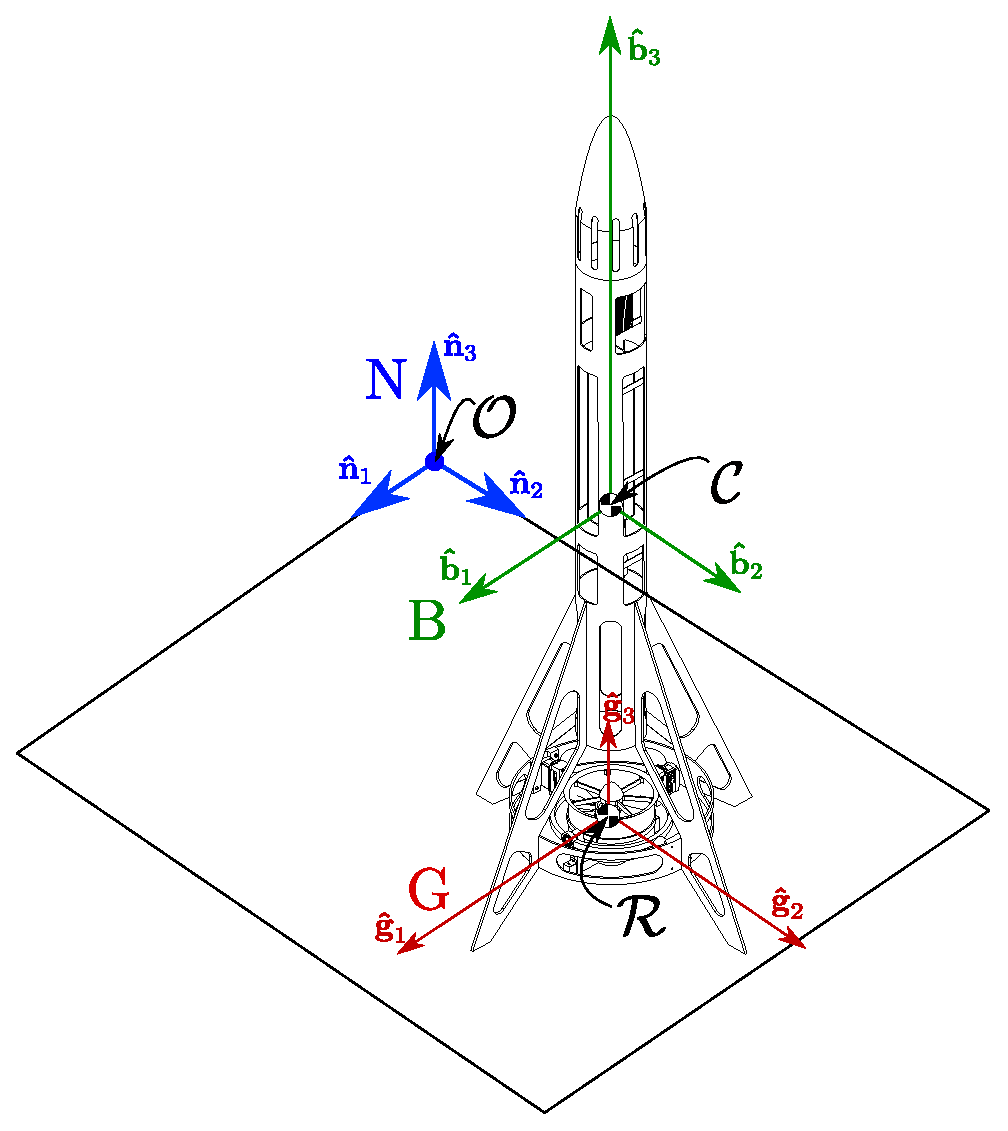
\includegraphics[width=0.52\textwidth]{fig/marcosDiagrama.eps}
	\caption{Marcos de referencia tomados para el análisis de cuerpo rígido. Por simplicidad se tomaron los centros de masa del cardán y del rotor como coincidentes en el punto $\ogn{R}$.}
\end{figure}

\newpage
\subsection{Notación}

La notación utilizada fue la del libro \textit{Rigid Body Dynamics of Mechanisms, Theoretical Basics} \cite{hahn2013rigid}. Se requirió un tratamiento algebraico explicito de los marcos de referencia y representación debido al caso especial de un \textit{gimballed rotor}. Este tratamiento facilitó la programación de la simulación y, en consecuencia, el control, el cual se volvería ambiguo y complejo con un tratamiento más común o simplificado.

\begin{description}
	\item[{\(\avec{r}_{\ogn{CO}}=[x,y,z]\)}] : Posición absoluta del centro de masa del vehículo léase ``posición de $\ogn{C}$ respecto $\ogn{O}$'')
	\item[{\(\avec{r}_{\ogn{RC}}\)}] : Posición del centro de masa del cardán respecto al centro de masa del vehículo
	\item[{\( \avec{\eta}=[\phi,\theta,\psi] \)}] : Ángulos de actitud del vehículo (Ángulos Euler)
	\item[\( \avec{\omega}_r^{\frm{G}} \)] : Velocidad angular del rotor del EDF representado en el marco $\frm{G}$ (dirección constante)
	\item[\( \avec{\omega}_\frm{BN}^\frm{B} \)] : Velocidad angular de $\frm{B}$ respecto a $\frm{N}$, representado en el marco $\frm{B}$.
	\item[\(  \alpha, \beta \)] : Ángulo de actuación de vectorización del EDF o ángulo de actitud del marco $\frm{G}$
	\item[{\( \delta   \)}] :  Ángulo de actuación de los dos flaps anti-roll
	\item[{\( m  \)}] :  Masa del vehículo sin rotor
	\item[{\( m_r  \)}] :  Masa del rotor
	\item[{\( \avec{g}  \)}] :  Aceleración de la gravedad
	\item[{\( \avec{F}^\frm{B} \)}] : Empuje del EDF representado en el marco $\frm{B}$ 
	\item[{\( \transform{NB}  \)}] :  Matriz de transformación de cosenos directores de un marco $\frm{B}$ a el marco $\frm{N}$
\end{description}

\textbf{Caracterización del EDF}
\begin{description}
	\item[{\( \tau_c  \)}] :  Torque efectivo de control del EDF
%	\item[{\( i  \)}] :  Corriente entregada al motor
	\item[{\( K_T  \)}] :  Constante de empuje del EDF
	\item[{\( K_Q  \)}] :  Coeficiente de torque viscoso de fricción
	\item[{\( Q  \)}] :  Torque viscoso de fricción
	\item[{\( \tau_r \)}] : Torque de reacción por el swirl de salida
\end{description}

\textbf{Caracterización del mecanismo anti-roll:}
\begin{description}
	\item[{\( K_{F_L}  \)}] : Coeficiente de lift de los flaps anti-roll
	\item[{\( K_{F_D}  \)}] : Coeficiente de drag de los flaps anti-roll
	\item[{\( F_L \)}] : Lift de los flaps anti-roll
	\item[{\( F_D \)}] : Drag de los flaps anti-roll
\end{description}

\textbf{Matriz de inercia:}
\begin{description}
	\item[{\(  \inertia{C}{B}  \)}] : Vehículo sin rotor respecto a $\ogn{C}$ representado en $\frm{B}$
	\item[{\(  \inertiarotor{R}{G}  \)}] : Rotor respecto a $\ogn{R}$ representado en $\frm{G}$
	\item[{\(  \inertia{\!\mathrm{g}R}{G}  \)}] : Cardán y motor sin rotor respecto a $\ogn{R}$ representado en $\frm{G}$
\end{description}



\subsection{Notación del álgebra a utilizar}

El producto escalar se definió como $\bigcdot$ para diferenciarlo de simple multiplicación vectorial ($\cdot$). $\skw{\omega}$ es la matriz skew del vector que reemplaza el producto vectorial ya que $\skw{r}\cdot v = r \times v$
\[
\skw{\omega}_{L R}^{L}=\left(\begin{array}{ccc}
0 & -\omega_{z L R}^{L}, & \omega_{y L R}^{L} \\
\omega_{z L R}^{L} & 0 &-\omega_{x L R}^{L} \\
-\omega_{y L R}^{L} &  \omega_{x L R}^{L} & 0
\end{array}\right)
\]

Se definió a $J_\ogn{C}^\frm{B}$ como la matriz de inercia respecto al punto $\ogn{C}$, representada en el marco $\frm{B}$: es decir, las componentes de la matriz de inercia están en la base de $\frm{B}$. Esto se puede escribir así:
\begin{IEEEeqnarray*}{c}
J_\ogn{C}^\frm{B} = J_{b1} \bvec{b}_1 + J_{b2} \bvec{b}_2 + J_{b3} \bvec{b}_3
\end{IEEEeqnarray*}

La derivada del término anterior respecto un marco $N$ quedó definida
$${}^\frm{N}\dot{J}_{\ogn{C}}^\frm{B} =\left.^\frm{N} \frac{\di J_\ogn{C}^\frm{B}}{\di t}  \right. = \transform{NB} \cdot \left.^\frm{B} \frac{\di J_\ogn{C}^\frm{B}}{\di t}  \right. $$


Se pueden demostrar las siguientes ecuaciones
\begin{IEEEeqnarray}{C}
\dottransform{RL} =\transform{RL}\cdot \skw{\omega}^\frm{L}_\frm{LR} =
\skw{\omega}^\frm{R}_\frm{LR}\cdot\transform{LR} = -\skw{\omega}^\frm{L}_\frm{LR}\cdot\transform{RL} \\
\transform{BN} = (\transform{NB})\tp =  (\transform{NB})^{-1} \quad \Rightarrow \quad \transform{NB} \cdot \transform{BN} = \eye
\end{IEEEeqnarray}

donde $\omega_{\frm{LR}}^{\frm{L}}$ es la velocidad angular vectorial del marco $\frm{L}$ con respecto a $\frm{R}$ representado en $\frm{L}$, $\transform{RL}$ es la matriz de cosenos directores que transforma una vector de una base ortogonal $\frm{L}$ a otra base ortogonal $\frm{R}$, y $\dottransform{RL}$ es la derivada de la matriz $\transform{RL}$ respecto $\frm{R}$.

\newpage

\subsection{Variables de estado}
Se obtuvieron las variables de estado de posición y velocidad donde $z$ positivo es alejándose de la tierra.
\[
\avec{r}_\ogn{CO}^\frm{N} = 
\begin{bmatrix}
x & y & z 
\end{bmatrix}, \qquad
\dot{\avec{r}}_\ogn{CO}^\frm{N} = 
\begin{bmatrix}
\dot{x} & \dot{y} & \dot{z}
\end{bmatrix} 
\]

El movimiento cuerpo rígido se describió por 3 ángulos de Euler (Cardán o Bryant en algunas bibliografías) $\phi, \theta$ y $\psi$ (roll, pitch, yaw respectivamente).
\begin{IEEEeqnarray}{C}
\avec{\eta} = \begin{bmatrix}
\phi  &  \theta &  \psi
\end{bmatrix}
\end{IEEEeqnarray}

\begin{figure}[ht!]
	\centering
	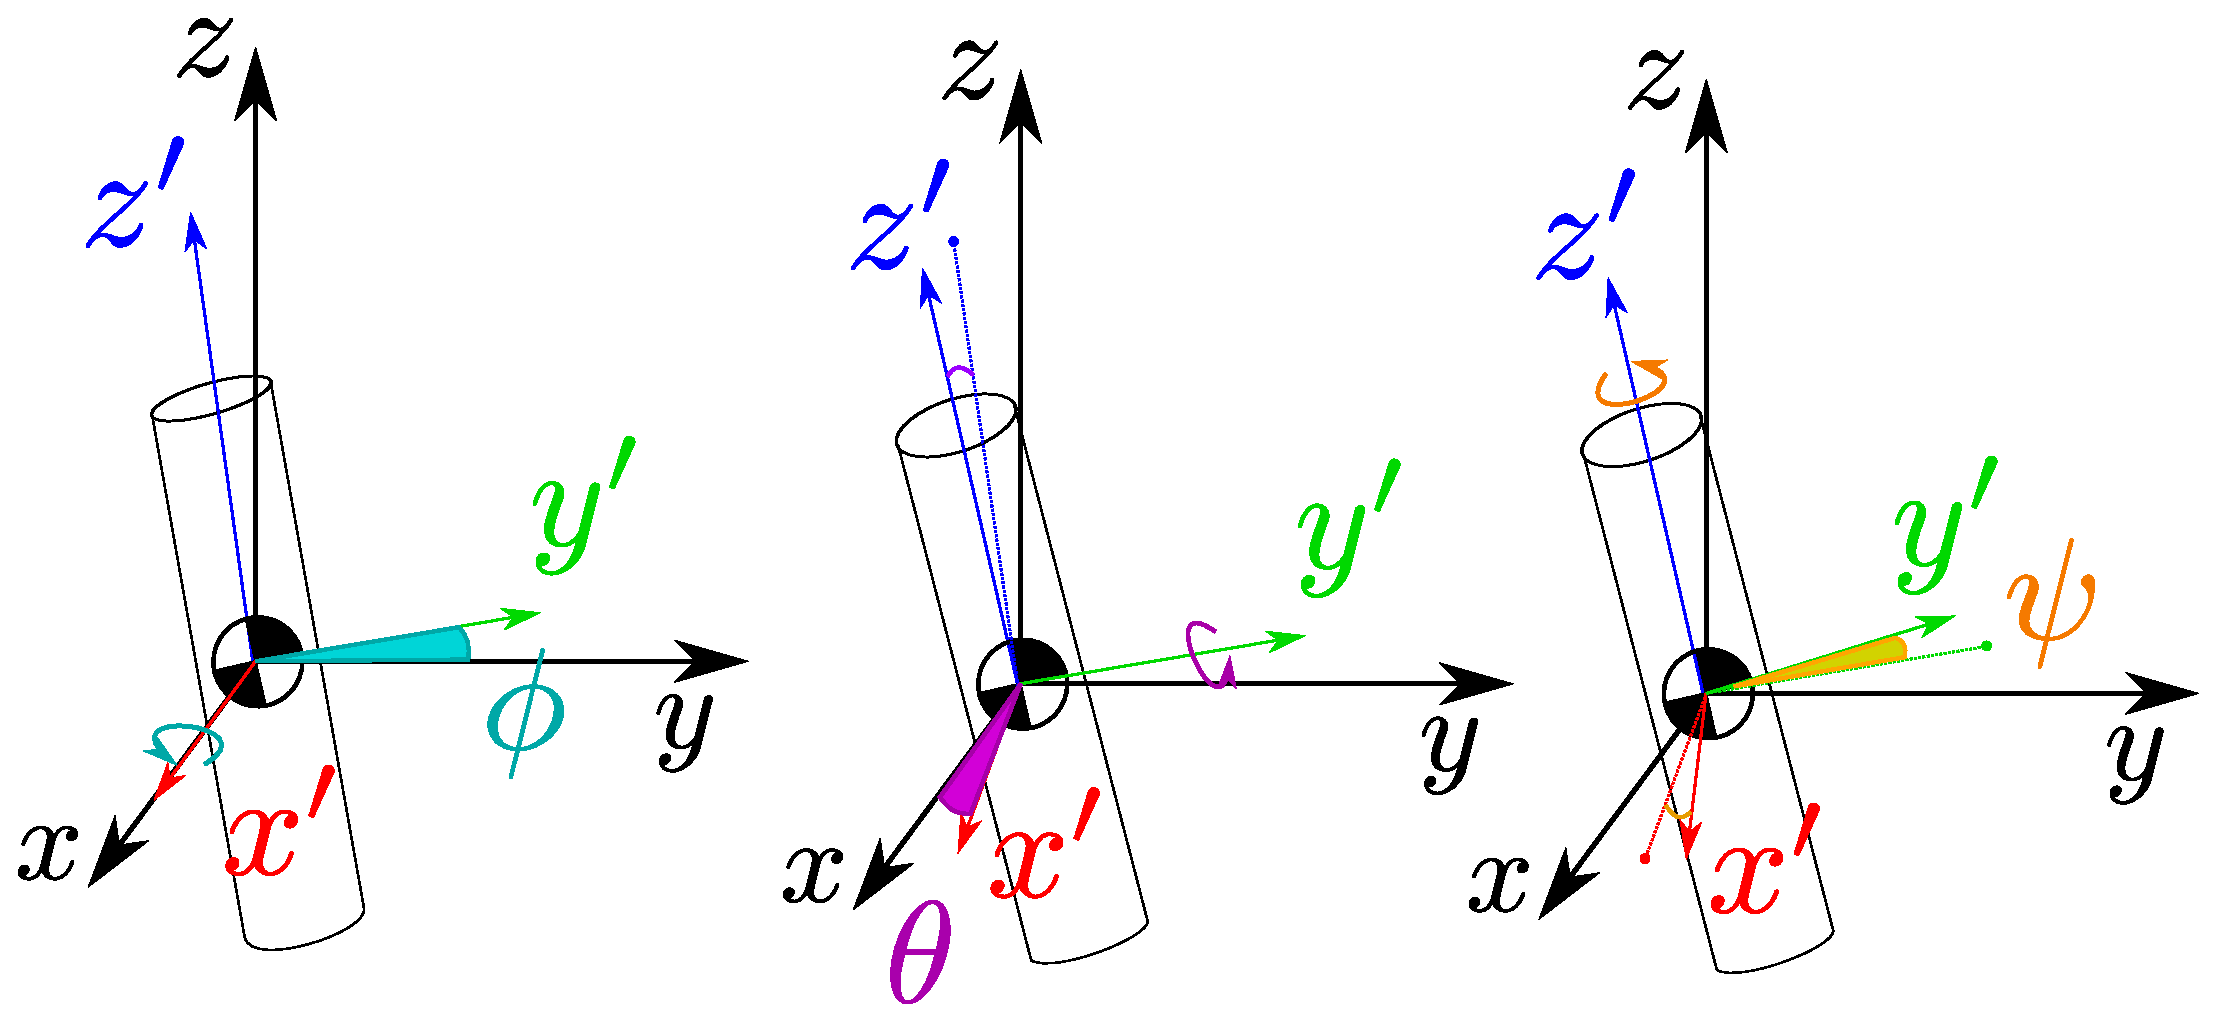
\includegraphics[width=0.8\textwidth]{fig/cuerpolibreGlobal_v2.eps}
	\caption{Diagrama mostrando las rotaciones de ángulo de euler en el orden que son efectuadas para describir el sistema. $\phi$ representa el pitch, $\theta$ el yaw y $\psi$ el roll. Se muestran las últimas posiciones de los ejes rotados con una linea punteada.}
\end{figure}


Los ángulos de la vectorización de la tobera fueron $\alpha$ y $\beta$. El ángulo $\delta$ correspondió a los actuadores que contrarrestan el roll del vehículo mediante dos flaps. Los ángulos $\alpha$ y $\beta$ describieron la dirección en la que está apuntando la tobera (equivalente a la orientación $\frm{G}$) respecto la dirección del vehículo (marco $\frm{B}$). $\omega_r=\omega_r^\frm{G}$ es la velocidad angular del rotor.

\medskip

Se definieron las variables de estado y el vector input, donde $F$ es la fuerza que hace la tobera sobre el vehículo (la cual depende de la velocidad del vehículo)\footnote{En el código $\phi$, $\theta$ y $\psi$ aparecen como \texttt{q,r,s}}
\begin{equation} \label{eq:ssVariables3D}
	\Cx = \left[
	\begin{array}{cccccccc}
		\avec{r}_\ogn{CO}^\frm{N} & \avec{\eta} &\dot{\avec{r}}_\ogn{CO}^\frm{N} &  \avec{\omega}_\frm{BN}^\frm{B} & \omega_r & \alpha & \beta & \delta
	\end{array}\right] \tp
\end{equation}
\begin{equation}\label{eq:ssInputs3D}
	\Cu = \begin{bmatrix}
		\tau_c & \dot{\alpha} & \dot{\beta} & \dot{\delta}
	\end{bmatrix} \tp
\end{equation}
En la próxima sección se buscará obtener el vector de variables de estado derivado en el tiempo $\dot{\Cx}$.

\subsection{Ecuaciones diferenciales} \label{subsec:modeloMatematico}

\def\scos{\operatorname{c}}
\def\ssin{\operatorname{s}}
Se definió la transformación de los ángulos euler con una matriz de transformación $\transform{BN}$ donde $\scos$ y $\ssin$ fueron las funciones coseno y seno, respectivamente.

\begin{equation} \label{eq:matrizTransfoVehiculo}
	\transform{BN} = \begin{bmatrix}
	\scos \theta \cdot \scos \psi & \scos \theta \cdot \ssin \psi & - \ssin \theta \\
	\ssin \phi \cdot \ssin \theta \cdot \scos \psi - \scos \phi \cdot \ssin \psi & \ssin\phi \cdot \ssin\theta \cdot \ssin\psi + \scos\phi\cdot\scos\psi & \ssin\phi \cdot \scos\theta \\
	\scos\phi \cdot \ssin\theta \cdot \scos\psi + \ssin\phi \cdot \ssin\psi\quad & \scos\phi \cdot \ssin\theta \cdot \ssin\psi - \ssin\phi \cdot \scos\psi \quad& \scos\phi \cdot \scos\theta
	\end{bmatrix}
\end{equation}
La transformación nos sirvió para poder pasar de la dinámica que está definida en el marco del vehículo $\frm{B}$ al marco $\frm{N}$ donde se obtienen las variables de estado que se desean controlar.

Se pudo obtener la velocidad en el marco del cuerpo
\begin{IEEEeqnarray}{rCl}
	\dot{\avec{r}}_\ogn{CO}^\frm{B} &= &\transform{BN} \cdot \dot{\avec{r}}_\ogn{CO}^\frm{N} 
\end{IEEEeqnarray}

La obtención de la velocidad angular del cuerpo se complicó por el hecho de que la razón de cambio de los ángulos de Euler no son vectores cartesianos, si no más bien parámetros que describen la orientación del cuerpo rígido en el espacio.\footnote{ Como bien sabemos la matriz de transformación $\tform$ solo es aplicable para transformar vectores cartesianos de una base ortogonal a otra. Los parámetros $\avec{\eta}$ conforman un vector de configuración, no un vector cartesiano!} Para relacionar la velocidad angular con $\avec{\eta}$ fue necesario utilizar la matriz de actitud cinemática $\attitude(\avec{\eta})$.

\begin{IEEEeqnarray}{c}
	\attitude(\avec{\eta}) = \left[\begin{array}{ccc}
	1 & \sin (\phi) \tan (\theta) & \cos (\phi) \tan (\theta) \\
	0 & \cos (\phi) & -\sin (\phi) \\
	0 & \sin (\phi) \sec (\theta) & \cos (\phi) \sec (\theta)
	\end{array}\right]
\end{IEEEeqnarray}

La matriz de actitud cinemática se usó para transformar 
\begin{IEEEeqnarray}{rCl}
	 \dot{\avec{\eta}}& = & \attitude(\avec{\eta}) \cdot  \avec{\omega}_\frm{BN}^\frm{N} \\
	\avec{\omega}_\frm{BN}^\frm{B} & = &\transform{BN}\cdot \avec{\omega}_\frm{BN}^\frm{N}
\end{IEEEeqnarray}
e inversamente
\begin{IEEEeqnarray}{rCl}
	\avec{\omega}_\frm{BN}^\frm{N} & = &\attitude^{-1}(\avec{\eta})\cdot \dot{\avec{\eta}} \\
\end{IEEEeqnarray}


La fuerza que impulsó al vehículo en el marco del cuerpo se obtuvo transformando del marco del cardán donde se conocen los componentes, al marco cuerpo. La matriz fue calculada reemplazando $\phi\equiv\alpha$, $\theta\equiv\beta$, y $\psi = 0$.
\begin{equation}
	\avec{F}^\frm{B} = \transform{BG} \cdot \avec{F}^\frm{G} 
\end{equation}

La aceleración del centro de masa del vehículo se midió en el marco del cuerpo $\frm{B}$ y fue igualada a  $\avec{F}$
\begin{equation}
	{}^\frm{B}\frac{\di }{\di t}\left( \dot{\avec{r}}_\ogn{CO}^\frm{B} \right) = \frac{1}{m+m_r} \cdot \avec{F}^\frm{B}
\end{equation}
luego obtenemos la aceleración en coordenadas globales
\begin{equation}
	\ddot{\avec{r}}_\ogn{CO}^\frm{N} =
	\transform{NB}\cdot {}^\frm{B}\frac{\di }{\di t}\left( \dot{\avec{r}}_\ogn{CO}^\frm{B} \right)- \avec{g}^\frm{N}
\end{equation}

Los momentos actuantes externos en el marco del vehículo respecto su centro de gravedad $\ogn{C}$ se calcularon en base al diseño de los flaps anti roll según~\cite{isaac2022mathematical}.
\todo{Se tiene que tratar el termino de la vorticidad aqui. Se puede suponer que la vorticidad forma parte del termino de flaps y que se modela como si fuera un offset del angulo de actuacion, es decir, cuando los flaps estan actuados en angulo cero va haber un momento debido a la vorticidad del flujo del EDF. Entonces a la ecuacion de abajo se le agrega un término constante al angulo del flap actuado para tomarlo en cuenta.}

\begin{equation}
	\avec{M}^\frm{B}_\ogn{C} = \skw{\avec{r}}_\ogn{RC}^\frm{B}\cdot \avec{F}^\frm{B} + \transform{BG} \cdot 
	\begin{bmatrix}
		0 \\
		0 \\
		\omega_r^2 K_{F_L}d_T\delta+\tau_r
	\end{bmatrix}  
\end{equation}

La aceleración angular en el marco $\frm{B}$ se obtuvó del desarrollo de la sección~\ref{ssec:ecuacionangular} del anexo.
\begin{equation}
	\hspace{-1cm}
{}^\frm{B}\frac{\di }{\di t} \left(\avec{\omega}_\frm{BN}^\frm{B} \right) =  \left(\inertia{C}{B}\right)^{-1} \cdot \left( - \skw{\avec{\omega}}_\frm{BN}^\frm{B} \cdot \inertia{C}{B}\cdot \avec{\omega}_{\frm{BN}}^{\frm{B}} - 
\transform{{BG}} \cdot\skw{\avec{\omega}}_\frm{GB}^\frm{G} \cdot \inertiarotor{R}{G}  \cdot \avec{\omega}_r^\frm{G} -
\skw{\avec{\omega}}_\frm{BN}^\frm{B} \cdot \inertiarotor{R}{G}  \cdot \avec{\omega}_r^\frm{G} -
\transform{{BG}}\cdot  \inertiarotor{C}{G} \cdot  {}^\frm{N} \dot{\avec{\omega}}_{\!r}^{\frm{G}} + \avec{M}_\ogn{C}^\frm{B} \right)
\end{equation}

El rotor y los servos son modelados como de primer orden por el momento. Su valor en las simulaciones fueron limitados por velocidad máxima según sus especificaciones.

Las ecuaciones diferenciales usadas para el control del vehículo fueron las siguientes
\begin{equation} \label{eq:ssDiffVariables3D}
	\dot{\Cx} = \left[
	\begin{array}{cccccccc}
		\dot{\avec{r}}_\ogn{CO}^\frm{N}& \dot{\avec{\eta}} &\ddot{\avec{r}}_\ogn{CO}^\frm{N} & {}^\frm{B}\frac{\di }{\di t} \left(\avec{\omega}_\frm{BN}^\frm{B} \right) & \dot{\omega}_r & \dot{\alpha} & \dot{\beta} & \dot{\delta}
	\end{array}\right] \tp~
\end{equation}


\subsection{Dinámica angular del vehículo}\label{ssec:ecuacionangular}

El momento angular del vehículo respecto de su centro de masa ($\ogn{C}$) y representado en el marco fijo-tierra $\frm{N}$ debió tomar en cuenta el momento angular por tener un cuerpo con velocidad lineal y angular propia. 

\begin{equation}
		L_{\ogn{C}}^{\frm{N}} = \underbrace{\transform{{NB}} \cdot J_{\ogn{C}}^{\frm{B}} \cdot \omega_{\frm{BN}}^{\frm{B}}}_{\text{Vehículo}} +
		\underbrace{\transform{{NG}}J_{\!g\ogn{R}}^{\frm{G}} \cdot \omega_\frm{GN}^\frm{G} +
		 m_{g}\cdot \skw{\avec{r}}^\frm{N}_\ogn{RC} \cdot\dot{\avec{r}}^\frm{N}_\ogn{RC} }_\text{Cardán \& EDF} + \underbrace{ \transform{NG} \cdot J_{\!r\ogn{R}}^\frm{G} \cdot \omega_{\!r}^\frm{G} + m_{r}\cdot \skw{\avec{r}}^\frm{N}_\ogn{RC} \cdot\dot{\avec{r}}^\frm{N}_\ogn{RC}}_\text{Rotor}
\end{equation}

Esta ecuación describió los efectos de tener un cardán con un rotor integrado acoplado al vehículo sin embargo algunos términos se pudieron considerar despreciables debido al diseño del cardán. 

Ambos gimbals del cardán tienen su eje de giro cercano a su centro de masa lo cual significó que la velocidad relativa entre los puntos $\ogn{R}$ y $\ogn{C}$ tuvieron poco impacto sobre los torques internos del vehículo. Se consideró que
\begin{equation}
\dot{\avec{r}}_\ogn{RC}  = 0
\end{equation}

La velocidad angular de los gimbals fue poca ya que su actuación ocurrió en el orden de la décima de grado lo cual implicó un bajo impacto del término del cardán cuando fue integrado en el tiempo. El término  $\transform{NG} \cdot J_{\!g\ogn{R}}^{\frm{G}} \cdot \omega_\frm{GN}^\frm{G}$ entonces pasó a formar parte de la inercia del resto del vehículo $\inertia{C}{B}$, el cual solo excluyó al rotor.



El momento angular quedó simplificado de la siguiente manera:


\begin{equation}
	L_{\ogn{C}}^{\frm{N}} = \transform{{NB}} \cdot \inertia{C}{B} \cdot \omega_{\frm{BN}}^{\frm{B}} +\transform{NG} \inertiarotor{R}{G} \cdot \omega_{\!r}^\frm{G}
\end{equation}

donde
\begin{description}
	\item[$\omega_{\!r}$] : velocidad del rotor
	\item[$\inertiarotor{R}{G}$] : matriz de inercia del rotor tomado alrededor de su centro de masa representado en coordenadas del marco cardán $\frm{G}$
\end{description}


Se derivó el momento angular con respecto a $\frm{N}$ y junto con $\inertia{C}{B} \approx \text{constante}$\footnote{La inercia del vehículo en su propio marco $\inertia{C}{B}$ fue constante excepto por las variaciones introducidas al agruparlo con el término del cardán $J_{\!g\ogn{C}}^\frm{B}$, el cual varió en función a la actuación $\alpha,\beta$.}

\begin{IEEEeqnarray*}{rCl}
	\hspace{-1cm}
^{\frm{N}}\dot{L}_{\ogn{C}}^{\frm{N}}  & = & ^{\frm{N}} \frac{\di}{\di~t}  \left(\transform{{NB}} \cdot \inertia{C}{B} \cdot \omega_{\frm{BN}}^{\frm{B}} + \transform{{NG}}\cdot \inertiarotor{R}{G} \cdot \omega_r^\frm{G} \right) \\
 & = & \dottransform{NB} \cdot\inertia{C}{B}\cdot \omega_{\frm{BN}}^{\frm{B}} + 
 \transform{{NB}} \cdot \underbrace{ {}^\frm{N}\dot{J}_{\ogn{C}}^\frm{B}}_{\approx~0}\cdot \omega_{\frm{BN}}^{\frm{B}} +
  \transform{{NB}} \cdot \inertia{C}{B}\cdot \dot{\omega}_{\frm{BN}}^{\frm{B}} + 
  \dottransform{NG}\cdot  \inertiarotor{R}{G} \cdot \omega_{\!r}^\frm{G} +
  \transform{{NG}}\cdot {}^\frm{N}\frac{\di}{\di~t}\left(\inertiarotor{R}{G}  \cdot \omega_r^\frm{G} \right)
\end{IEEEeqnarray*}
la derivada de la inercia del cuerpo se anuló y luego se aplicó la regla de la cadena a la derivada
%\transform{{NG}}\cdot {}^\frm{N}\frac{\di}{\di t}\left( \inertiarotor{R}{G}  \cdot \omega_r^\frm{G} \right)
\begin{IEEEeqnarray*}{rCl}
	\hspace{-1cm}
^{\frm{N}}\dot{L}_{\ogn{C}}^{\frm{N}}  &=&\dottransform{NB} \cdot J_{\ogn{C}}^\frm{B}\cdot \omega_{\frm{BN}}^{\frm{B}} + 
\transform{{NB}} \cdot \inertia{C}{B}\cdot \dot{\omega}_{\frm{BN}}^{\frm{B}} + 
\dottransform{NG}\cdot \inertiarotor{R}{G}  \cdot \omega_r^\frm{G} +
\transform{{NG}}\cdot {}^\frm{N}\frac{\di}{\di t}\left( \inertiarotor{R}{G}  \cdot \omega_r^\frm{G} \right) \\
&=&\transform{{NB}} \cdot \skw{\omega}_\frm{BN}^\frm{B} \cdot \inertia{C}{B} \cdot \omega_{\frm{BN}}^{\frm{B}} + 
\transform{{NB}} \cdot \inertia{C}{B}\cdot \dot{\omega}_{\frm{BN}}^{\frm{B}} + 
\transform{{NG}} \cdot\skw{\omega}_\frm{GN}^\frm{G} \cdot\inertiarotor{R}{G}  \cdot \omega_r^\frm{G} +
\transform{{NG}}\cdot \left( {}^{\frm{N}} \dot{J}_{\! r\ogn{R}}^\frm{G} \cdot \omega_{\!r}^{\frm{G}} + 
 \inertiarotor{R}{G} \cdot {}^\frm{N} \dot{\omega}_{\!r}^{\frm{G}}  \right)
\end{IEEEeqnarray*}
donde $ \dot{J}_{\! r\ogn{R}}^\frm{G}$ se consideró despreciable por la geometría ligera del conjunto cardán y por actuaciones pequeñas (mencionadas anteriormente).

\medskip

Como el rotor fue fijado al vehículo alrededor de un punto cercano a $\ogn{R}$ y  el movimiento del gimbal fue restringido por los actuadores se supuso que el rotor fue parte del cuerpo rígido del vehículo y se planteo su momento angular como un vector libre. Así se logró igualar $\inertiarotor{R}{G} \equiv \inertiarotor{C}{G} = \inertiarotor{}{G}$, y por extensión, $J_\ogn{R}^{\frm{B}} \equiv J_\ogn{C}^{\frm{B}} $. 




\begin{IEEEeqnarray*}{rCl}
&=&\transform{{NB}} \cdot \skw{\omega}_\frm{BN}^\frm{B} \cdot \inertia{C}{B} \cdot \omega_{\frm{BN}}^{\frm{B}} + 
\transform{{NB}} \cdot \inertia{C}{B} \cdot \dot{\omega}_{\frm{BN}}^{\frm{B}} + 
\transform{{NG}} \cdot\skw{\omega}_\frm{GN}^\frm{G} \cdot \inertiarotor{}{G}  \cdot \omega_r^\frm{G} +
\transform{{NG}}\cdot  \inertiarotor{}{G} \cdot  {}^\frm{N} \dot{\omega}_{\!r}^{\frm{G}}
\end{IEEEeqnarray*}
luego se multiplicó por $\transform{BN}$


\begin{IEEEeqnarray*}{rCl}
\transform{BN} \sum_i M_{i\ogn{C}}^\frm{N}=\sum_i M_{i\ogn{C}}^\frm{B}&=& \skw{\omega}_\frm{BN}^\frm{B} \cdot \inertia{C}{B}\cdot \omega_{\frm{BN}}^{\frm{B}} + 
\inertia{C}{B}\cdot \dot{\omega}_{\frm{BN}}^{\frm{B}} + 
\transform{{BG}} \cdot\skw{\omega}_\frm{GN}^\frm{G} \cdot \inertiarotor{}{G}  \cdot \omega_r^\frm{G} +
\transform{{BG}}\cdot  \inertiarotor{}{G} \cdot  {}^\frm{N} \dot{\omega}_{\!r}^{\frm{G}}  %\transform{BN} \cdot {}^\frm{N}\dot{L}^\frm{N}_\ogn{C}
\end{IEEEeqnarray*}
entonces
\begin{IEEEeqnarray*}{rCl}
\inertia{C}{B}\cdot \dot{\omega}_{\frm{BN}}^{\frm{B}} & = & - \skw{\omega}_\frm{BN}^\frm{B} \cdot \inertia{C}{B}\cdot \omega_{\frm{BN}}^{\frm{B}} - 
\transform{{BG}} \cdot\skw{\omega}_\frm{GN}^\frm{G} \cdot \inertiarotor{}{G}  \cdot \omega_r^\frm{G}-
\transform{{BG}}\cdot \inertiarotor{}{G} \cdot  {}^\frm{N} \dot{\omega}_{\!r}^{\frm{G}} + \sum_i M_{i\ogn{C}}^\frm{B}
\end{IEEEeqnarray*}
donde $\omega_\frm{GN}^\frm{G} =\omega_\frm{GB}^\frm{G} + \omega_\frm{BN}^\frm{G} =\omega_\frm{GB}^\frm{G} + \transform{GB} \omega_\frm{BN}^\frm{B} $
%\todo{Esto está bien? el término $ \skw{\omega}_\frm{BN}^\frm{B} \cdot \inertiarotor{}{G}  \cdot \omega_r^\frm{G}$ nos hace ruido}

\vspace{1cm}

se continuó el desarrollo matemático simplificando términos
\begin{IEEEeqnarray*}{rCl}
\hspace{-1cm}
\inertia{C}{B}\cdot \dot{\omega}_{\frm{BN}}^{\frm{B}} & = & - \skw{\omega}_\frm{BN}^\frm{B} \cdot \inertia{C}{B}\cdot \omega_{\frm{BN}}^{\frm{B}} - 
\transform{{BG}} \cdot\skw{\omega}_\frm{GB}^\frm{G} \cdot \inertiarotor{}{G}  \cdot \omega_r^\frm{G} -
\transform{{BG}}\transform{{GB}} \cdot\skw{\omega}_\frm{BN}^\frm{B} \cdot \inertiarotor{}{G} \cdot \omega_r^\frm{G} -
\transform{{BG}}\cdot  \inertiarotor{}{G} \cdot  {}^\frm{N} \dot{\omega}_{\!r}^{\frm{G}} + \sum_i M_{i\ogn{C}}^\frm{B} \\
& = & - \skw{\omega}_\frm{BN}^\frm{B} \cdot \inertia{C}{B}\cdot \omega_{\frm{BN}}^{\frm{B}} - 
\transform{{BG}} \cdot \skw{\omega}_\frm{GB}^\frm{G} \cdot \inertiarotor{}{G}  \cdot \omega_r^\frm{G} -
 \skw{\omega}_\frm{BN}^\frm{B} \cdot \inertiarotor{}{G}  \cdot \omega_r^\frm{G} -
\transform{{BG}}\cdot  \inertiarotor{}{G} \cdot  {}^\frm{N} \dot{\omega}_{\!r}^{\frm{G}} + \sum_i M_{i\ogn{C}}^\frm{B} \\
\end{IEEEeqnarray*}
obteniendosé ${}^\frm{N}\dot{\omega}_r^\frm{G} = \transform{GN}\cdot {}^\frm{G}\dot{\omega}_r^\frm{G} = \transform{GN} \cdot  \dot{\omega}_r \bvec{g}_3$
%\todo{$\transform{GN}$ debería ser $\transform{NG}$ posiblemente}


\section{Desarrollo de software}

La decisión de software a utilizar dependió del controlador, poder de cálculo disponible, interfases de periféricos y funcionalidad deseada.

\medskip

Dado el uso de una Raspberry Pi,\footnote{La Raspberry Pi provee un entorno con Linux instalado que permite la programación con virtualmente cualquier lenguaje de programación en existencia.} el lenguaje de programación elegido fue \textbf{Go} (Golang) debido a los siguientes puntos

\begin{description}
    \item[Seguro] - Modelo de memoria Go, sistema de tipado fuerte\footnote{Hoy en día hay pocos lenguajes con sistemas de tipos fuertes. Contrario a la creencia popular, C y C++ ambos son tipados débilmente.}
    \item[Simple] - Claridad de sintaxis
    \item[Concurrencia] - Crear \glsplural{corrutina} es simple, paralelizar corrutinas es trivieal
    \item[Rendimiento] - Superior a Python, Java y Matlab. Comparable a C. Esto también implica un menor consumo de energía
    \item[Estable] - \textit{The Go 1 promise} (La promesa Go 1)
    \item[Comprobado] -  Usado en sistemas de alto-riesgo/alta-complejidad (Kubernetes, Docker, Go-HEP)
    \item[Portable] - Todos los programas Go compilan a código nativo (código de máquina) para cualquier arquitectura y sistema operativo. Incluso se puede programar microcontroladores (TinyGo)
\end{description}

\subsection{Flujo de control}
\begin{figure}[!htb]
    \centering
    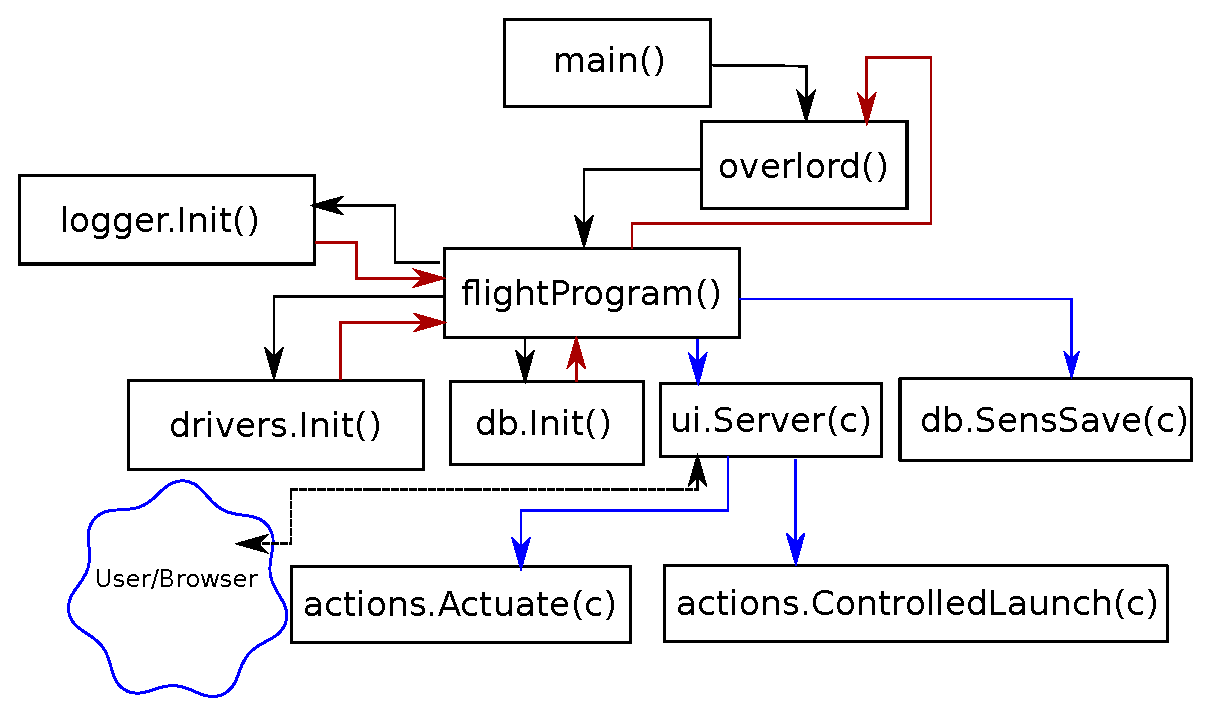
\includegraphics[width=0.7\textwidth]{fig/cfg_flightprogram.eps}
    \caption{Gráfico de flujo de control (CFG) del programa de vuelo. Las lineas de flujo azules son corrutinas independientes al programa principal. Las lineas negras son flujo del programa principal. Las lineas rojas son flujo del programa principal al encontrar un error.}
    \label{fig:flightProgram}
\end{figure}

Se ilustra el flujo de control a grandes rasgos usando un CFG en la figura \ref{fig:flightProgram}. El programa principal corrió la rutina \texttt{overlord} que a su vez comandó \texttt{flightProgram} y esperó que esta devuelva control a \texttt{overlord}. El propósito de \texttt{overlord} fue guardar el estado del vehículo y ante una falla irrecuperable en \texttt{flightProgram}, terminar con todas las corrutinas generadas por \texttt{flightProgram} y sus afiliadas y a su vez reiniciar \texttt{flightProgram} nuevamente con el último estado antes de la falla.


\subsection{Interfaz con hardware}

Como se mencionó anteriormente, la computadora elegida tiene varios puertos que sirviern como interfases con periféricos, entre ellos 

\begin{itemize}
    \item ADC (sensores)
    \item Generadores de PWM (para actuadores)
    \item Blinkenlights
\end{itemize}

Para la interacción del software con el hardware se usó la librería \href{https://periph.io}{periph.io}. Esta librería permitió la interacción a través de los puertos de comunicación de la Raspberry Pi. Los drivers para los periféricos fueron programados según la información dada en las datasheet.


\subsection{Implementación}

Al momento de escribir el presente informe el programa de vuelo tuvo 3540 líneas de lógica, de las cuales 1680 correspondieron a los drivers de control de periféricos. Se logró controlar la actuación de hasta 12 señales PWM y en simultaneo leer 16 señales de telemetría y guardar a archivo en una tarjeta SD a 1200 muestras por segundo (cada canal). 1060 líneas de código fueron dedicadas a la interfaz de usuario para facilitar el control del vehículo desde un browser, como por ejemplo Firefox.

\subsection{Debugging}

En junio 2021 se halló un bug en el software. Al cabo de cierto tiempo entraba en un estado degenerado el sistema donde no respondía a inputs de usuario ni a señales del sistema operativo. Debido a los periféricos usados la última señal mandada al actuador se quedaba fija y era imposible retornar el sistema a un estado seguro sin terminar el programa forzosamente y reiniciarlo. 

Se sospechaba que el bug era causa de una falla en el kernel de Linux para computadoras ARM o corrupción de memoria causada por el garbage collector de Go. Debido a la configuración de la computadora y las herramientas disponibles para Go era dificil debuggear. El debugger nativo de Go (Delve) no funcionaba aún en procesadores ARM de 32 bits y el detector de carreras de Go tampoco estaba disponible para procesadores ARM. Se pasó 6 meses investigando intermitentemente y hablando con expertos en software y hardware.

En enero 2022 se encontró el mismo comportamiento observado durante el bug mientras se desarrollaba un proyecto no asociado a este trabajo. En este software el estado degenerado era causado por una condición de carrera, específicamente era el caso de una \gls{datarace}. Con este conocimiento se modificó el programa de vuelo para que pueda correr en un entorno de computadora desktop. Para lograr esto se programó un mock de la escritura I2C que fue facilitado por el uso de \textit{interfaces} en Go. Esta modificación permitió al detector de carreras de Go encontrar condiciones de carrera en el programa de vuelo. Se encontraron y se arreglaron 2 condiciones de carreras causadas por error de programador debido al uso equivocado de mutexes.

Aún así el error persistía y el programa seguía encontrandosé en el estado degenerado. Se optó por reescribir el programa de cero y aplicando patrones de diseño más estrictos y seguros. Al cabo de un mes se había reescrito el programa de vuelo de la empresa y el bug no volvió a resurgir en el desarollo. Esto se puede deber a que se redujo el uso de librerias de terceros y la cantidad de líneas de código totales bajó de 700.000 a tan solo 30.000, incluyendo dependencias de terceros3. Excluyendo las liberías de terceros, la base de código era de tan solo 2100 líneas e incluía el frontend (interfaz con el usuario).




\subsection*{Agradecimientos}
Dan Etenberg por hacer todo posible. Ben Romarowski por ayuda con la dinámica de cuerpo rígido y aerodinámica de los álabes.




\bibliography{tex/biblio} % Indica archivo
\bibliographystyle{plainnat} %estilo de bibliografía
% \bibliographystyle{unsrtnat}
%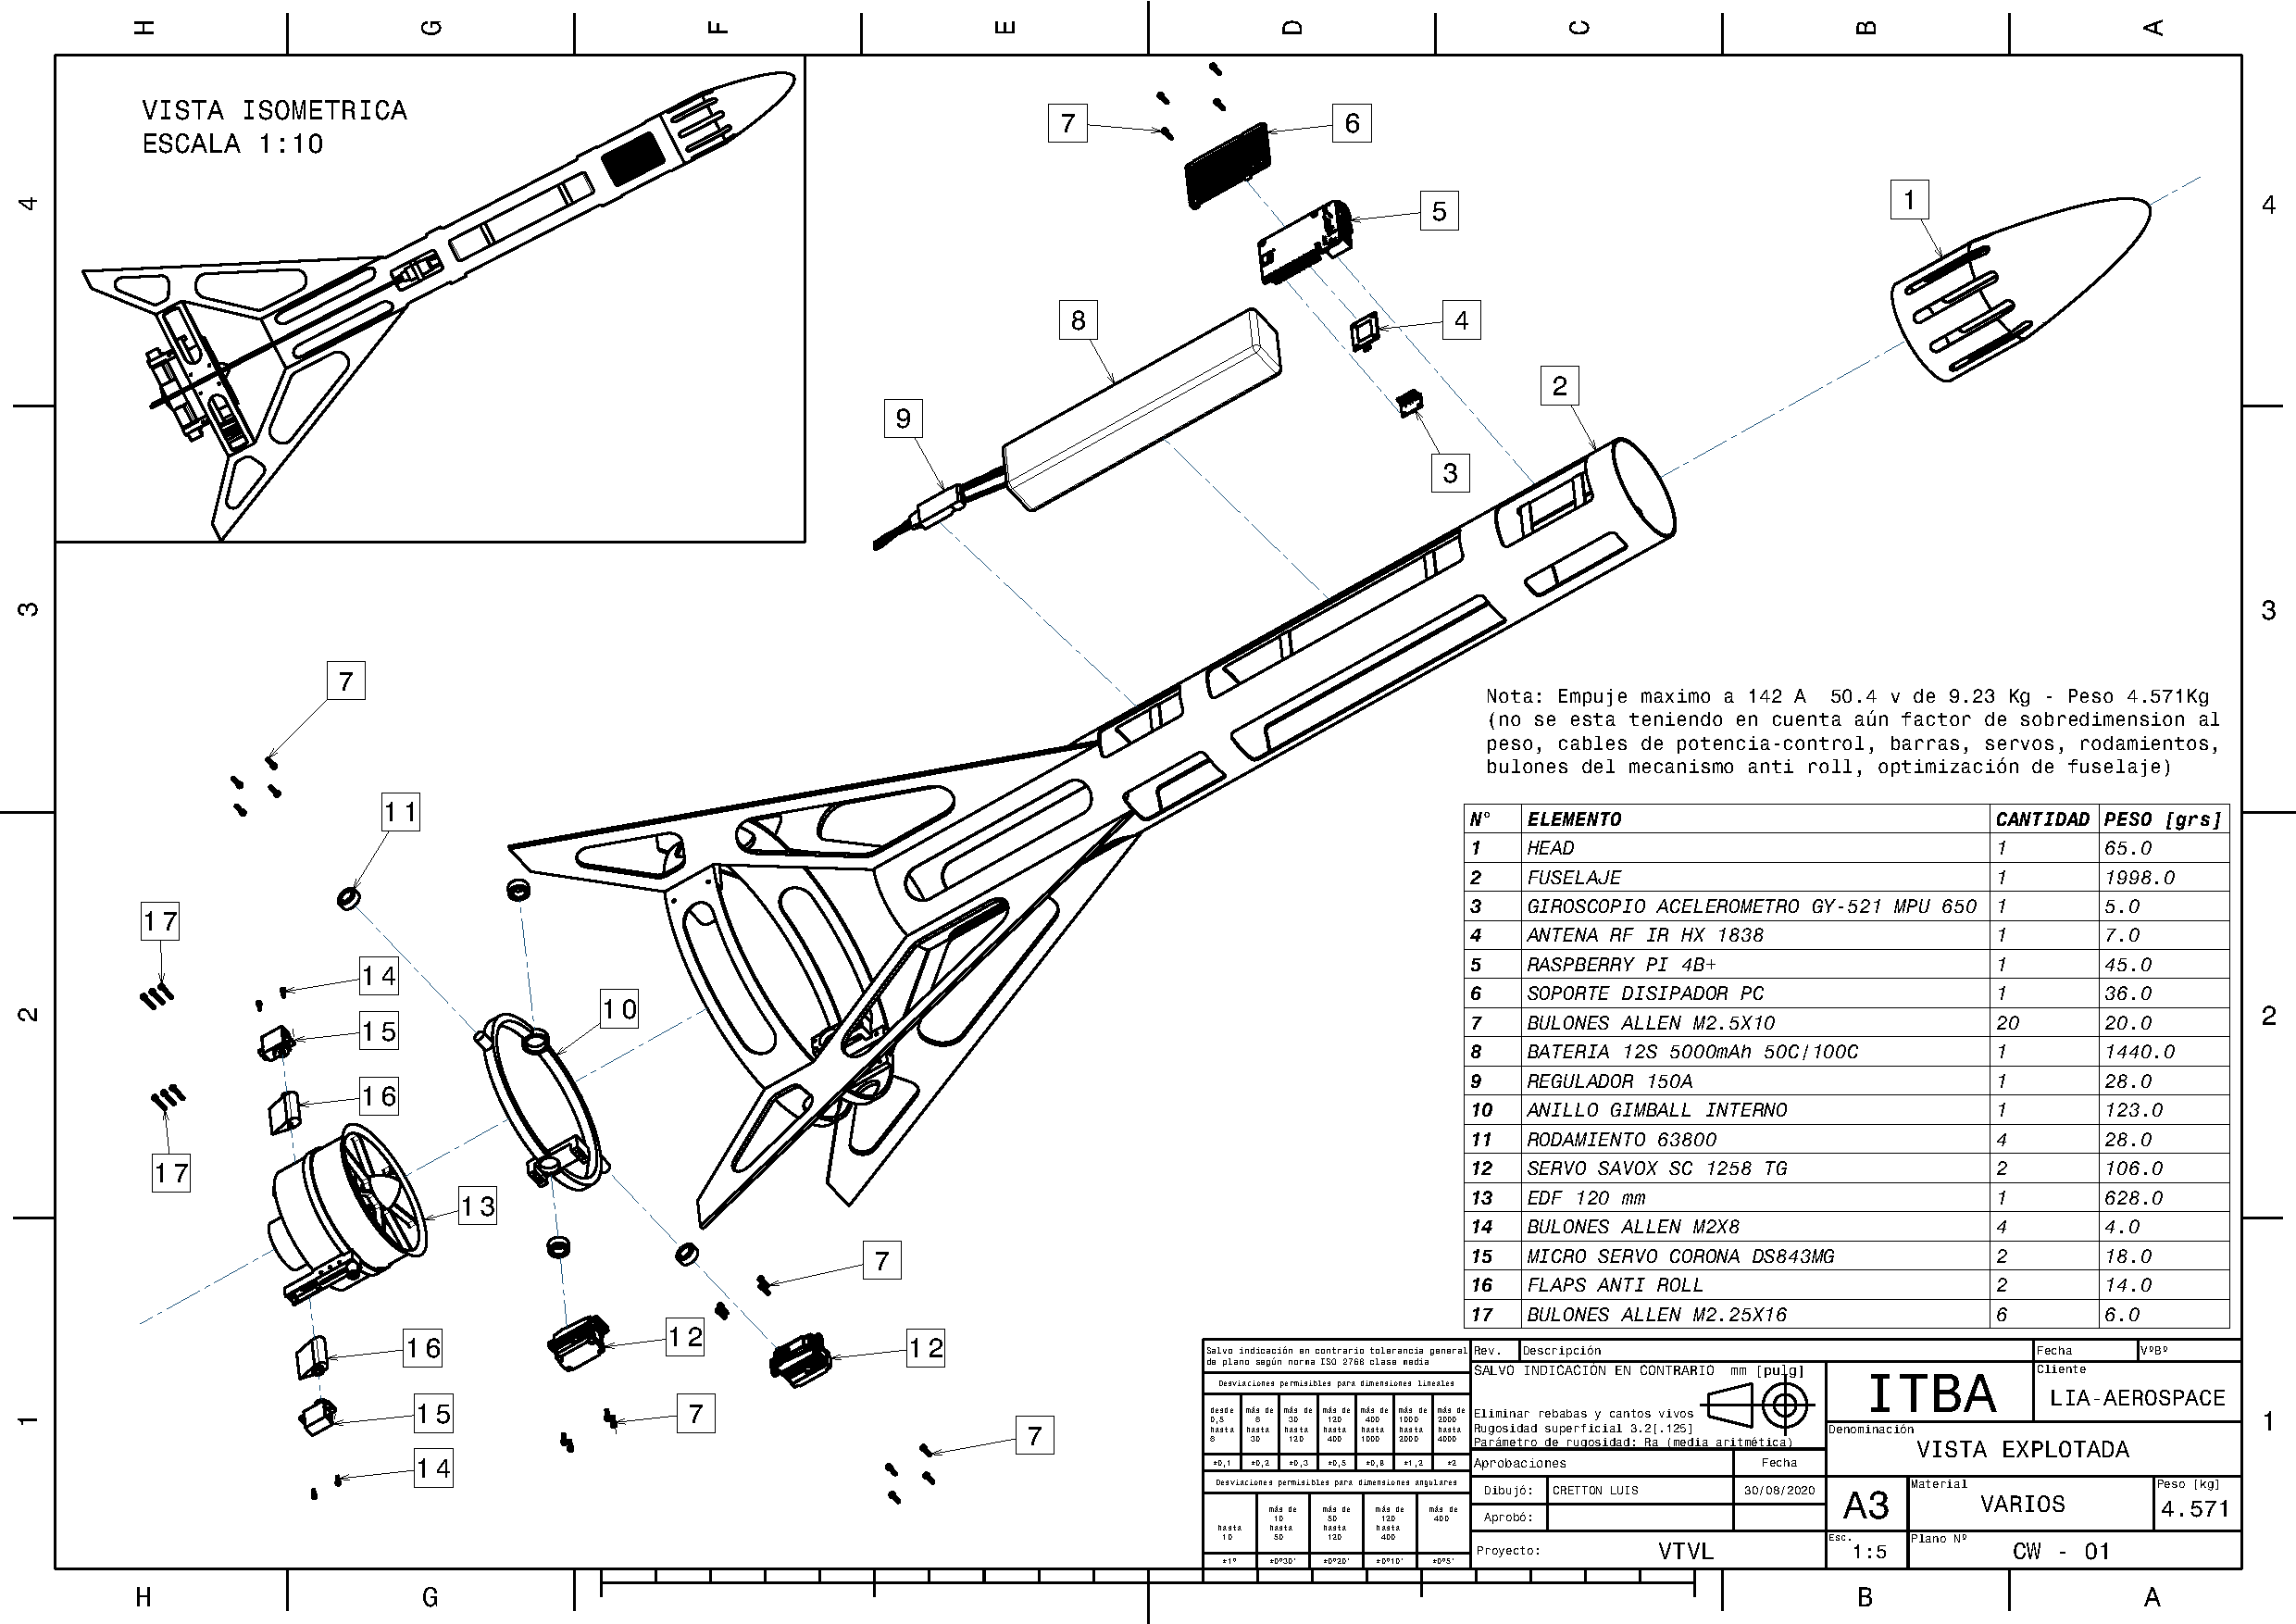
\includepdf[fitpaper=false,landscape]{pdf/Vistaexplotada5.pdf}
\end{document}
